\documentclass[a4paper,10pt]{article}

% ── Packages ──────────────────────────────────────────────────────────────────
\usepackage[
a4paper,
top=0.4cm,
bottom=0.4cm,
left=0.5cm,
right=0.5cm
]{geometry}

\usepackage[T1]{fontenc}
\usepackage[utf8]{inputenc}
\usepackage[sfdefault]{inter}
\usepackage{textcase}
\usepackage{graphicx}
\usepackage{tikz}
\usepackage{adjustbox}
\usepackage{fontawesome5}
\usepackage{array}
\usepackage{tabularx}
\usepackage{parskip}
\usepackage{titlesec}
\usepackage{xcolor}
\usepackage{microtype}
\usepackage{hyperref}

\pagestyle{empty}
\setlength{\parindent}{0pt}
\setlength{\parskip}{0pt}
\setlength{\topskip}{0pt}

% ── Colors ────────────────────────────────────────────────────────────────────
\definecolor{linkblue}{RGB}{0,102,255}
\definecolor{textblack}{RGB}{0,0,0}

% ── Hyperlink styling ─────────────────────────────────────────────────────────
\hypersetup{
colorlinks=true,
urlcolor=linkblue,
linkcolor=linkblue
}

% ── Section styling (Black Theme) ────────────────────────────────────────────
\titleformat{\section}
{\large\bfseries\color{textblack}}
{}{0em}{\MakeTextUppercase}[\vspace{-6pt}]

\titlespacing{\section}{0pt}{2pt}{0pt}

% ── Columns ───────────────────────────────────────────────────────────────────
\newcolumntype{L}{>{\raggedright\arraybackslash}p{3.2cm}}
\newcolumntype{M}{>{\raggedright\arraybackslash}p{12.3cm}}
\newcolumntype{G}{>{\raggedleft\arraybackslash}p{3.5cm}}
\newcolumntype{W}{>{\raggedright\arraybackslash}p{16.0cm}}

\renewcommand{\arraystretch}{0.95}

\begin{document}
\color{textblack}

% ── Header ────────────────────────────────────────────────────────────────────
\begin{minipage}[c]{0.72\linewidth}

{\fontsize{28}{30}\selectfont \textbf{Kartavya Suryawanshi}}\\[-2pt]

\normalsize
\faMapMarker*\ IIT Mandi, Kamand, Himachal Pradesh, India \\[-6pt]

\faPhone\ +91 86689 44955
\quad$\vert$\quad
\faEnvelope\ \href{mailto:b24199@students.iitmandi.ac.in}{\textcolor{linkblue}{b24199@students.iitmandi.ac.in}} \\[-6pt]

\faLinkedin\ \href{https://www.linkedin.com/in/kartavya-suryawanshi-918753320/}{\textcolor{linkblue}{LinkedIn}}
\quad$\vert$\quad
\faGithub\ \href{https://github.com/Kartavya728}{\textcolor{linkblue}{GitHub}} \\[-6pt]

Date of Birth: 28.07.2006
\quad$\vert$\quad
Place of Birth: Pune, Maharashtra, India
\quad$\vert$\quad
Nationality: Indian

\end{minipage}
\hfill
\begin{minipage}[c]{0.25\linewidth}
\raggedleft

\begin{tikzpicture}
\node[
fill=gray!12,
rounded corners=4pt,
draw=gray!45,
line width=1pt,
inner sep=1pt
]
{
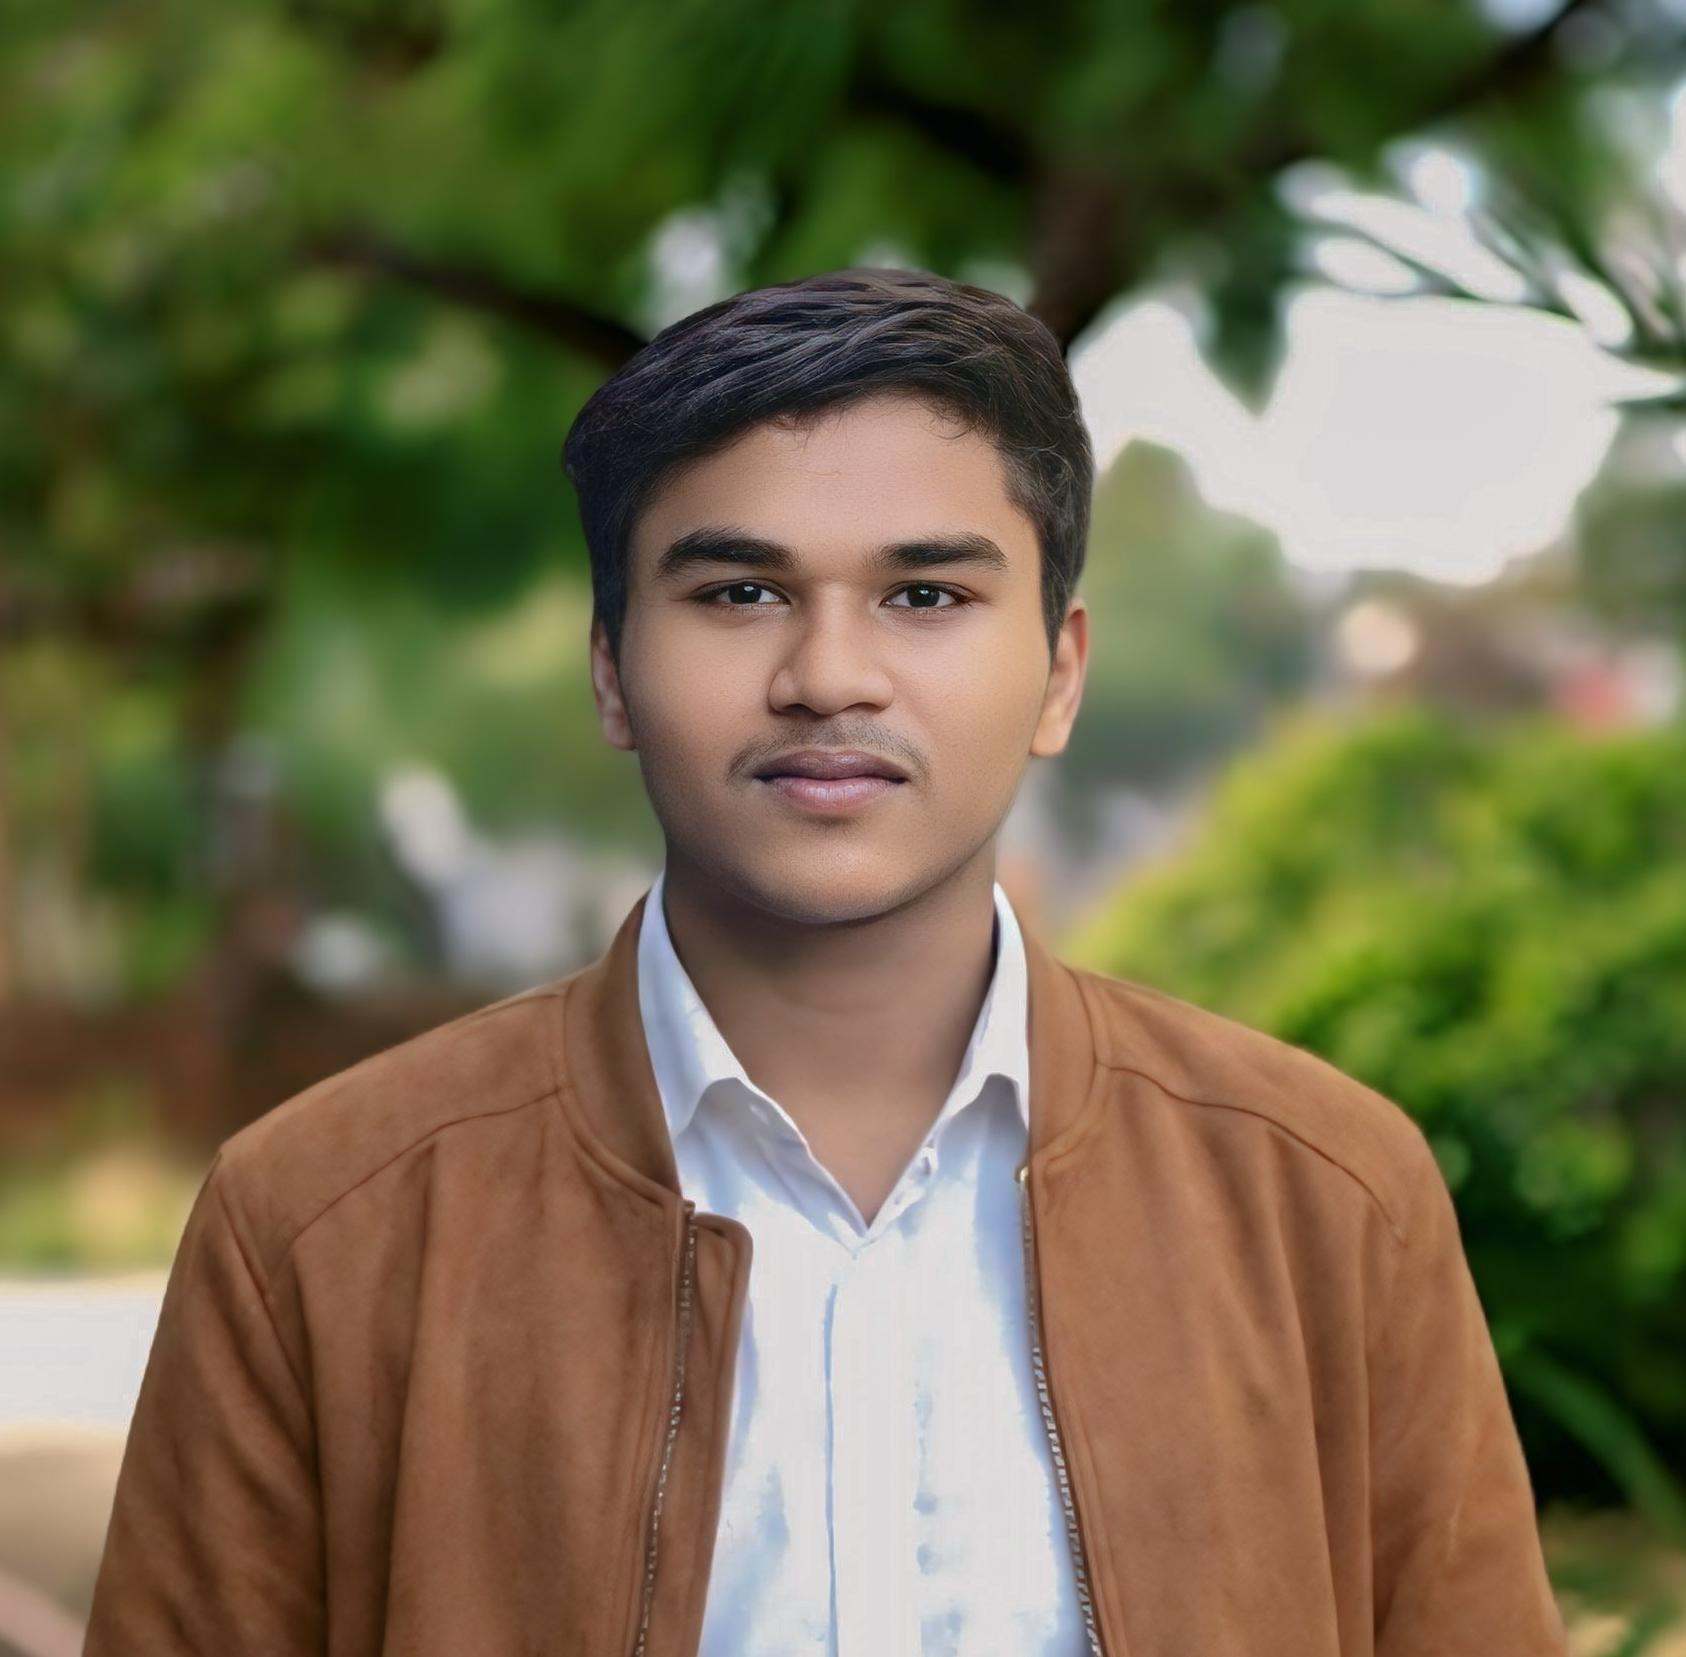
\includegraphics[width=2.8cm,height=2.8cm,keepaspectratio]{crop_profile.jpg}
};
\end{tikzpicture}

\end{minipage}

\vspace{1pt}
\noindent\rule{\linewidth}{0.8pt}

% ── Higher Education ──────────────────────────────────────────────────────────
\section*{Higher Education}
\noindent\rule{\linewidth}{0.6pt}

\begin{tabular}{L M G}
10/2026 -- 03/2027 & \textbf{Technical University of Munich (TUM)}, Germany & \\
& Exchange Student (TUMexchange) & \\
& \textit{School of Computation, Information and Technology (CIT -- Informatics)} & \\
2024 -- present & \textbf{Indian Institute of Technology Mandi (IIT Mandi)}, India & \\
& B.Tech.\ in Data Science \& Engineering (DSE) & \textit{CGPA: 9.27 / 10.00} \\
& \textit{\textbf{Relevant Coursework:}} Data Structures \& Algorithms, Machine Learning, Deep Learning, Computing Systems for Data Processing, Matrix Computations, Linear Algebra, Mathematical Foundations of Data Science, Data Handling \& Visualization, Computer Organization &
\end{tabular}

% ── School Education ──────────────────────────────────────────────────────────
\section*{School Education}
\noindent\rule{\linewidth}{0.6pt}

\begin{tabular}{L M G}
2021 -- 2023 & \textbf{Jadhavar Jr.\ College}, Pune, Maharashtra, India & \\
& Higher Secondary Certificate (Class XII) --- HSC Board & \textit{Aggregate: 86.0\%} \\
2016 -- 2021 & \textbf{NAJ Academy High School}, Murud Janjira, Raigad, Maharashtra, India & \\
& Secondary School Certificate (Class X) --- SSC Board & \textit{Aggregate: 91.4\%} \\
\end{tabular}

% ── Professional Experience ───────────────────────────────────────────────────
\section*{Professional Experience}
\noindent\rule{\linewidth}{0.6pt}

\begin{tabular}{L M G}
06/2026 -- 07/2026 & \textbf{Nomura Real Estate Holdings}, Tokyo, Japan & \\
& \textbf{Data Analytics Intern} & \\
& Analysed enterprise collaboration and productivity using MS Viva Insights and Power BI. Developed data dashboards to generate insights supporting strategic business decisions. & \\
08/2025 -- 12/2025 & \textbf{Finance Department, IIT Mandi}, India & \\
& \textbf{Full Stack Developer} & \\
& Developed and deployed a web portal for institutional fund management, improving administrative workflows through digital automation. &
\end{tabular}

% ── Projects ──────────────────────────────────────────────────────────────────
\section*{Projects}
\noindent\rule{\linewidth}{0.6pt}

\begin{tabular}{L M G}
2025 & \textbf{LunaDEM} --- Lunar Digital Elevation Model Library & \href{https://github.com/Kartavya728/LunaDEM}{\textcolor{linkblue}{[GitHub]}}~\href{https://pypi.org/project/lunadem/0.1.1/}{\textcolor{linkblue}{[PyPI]}} \\
& Python library for lunar DEMs; processed 500+ images at 5\,m resolution, 60\% faster. & \\
2025 & \textbf{Smarts Scribe} --- Multimodal Lecture Intelligence Platform & \href{https://github.com/Kartavya728/Smart-Scribes}{\textcolor{linkblue}{[GitHub]}} \\
& AI system for lecture summaries \& Q\&A across video, audio, PDFs; RAG on 10k+ segments. & \\
2026 & \textbf{LokMitra AI} --- AI Voice Assistant for Government Services & \href{https://github.com/Kartavya728/LokMitra-AI}{\textcolor{linkblue}{[GitHub]}}~\href{https://modest-reflection-production-893c.up.railway.app/}{\textcolor{linkblue}{[Live]}} \\
& Multilingual (10+ languages) voice assistant; RAG on 100+ docs, $\sim$2\,s latency. &
\end{tabular}

% ── Achievements ──────────────────────────────────────────────────────────────
\section*{Achievements}
\noindent\rule{\linewidth}{0.6pt}

\begin{tabular}{L W}
2025 & \textbf{Winner} --- NASA Space Apps Challenge: 1st among 100+ teams, Chandigarh regional; \textit{Astrogenesis} --- NASA Bioscience Research Engine using RAG. \\
2025 & \textbf{Winner} --- iHub Multimodal AI Hackathon: 1st among 1,600+ teams for \textit{Smarts Scribe}; led 3-member team end-to-end. \\
2026 & \textbf{Winner} --- Hack 60, HCLTech $\times$ IIT Mandi: 1st place, DL Audio Anti-Spoofing track. \\
2026 & \textbf{1st Runner-Up} --- Frosthack IIT Mandi: 2nd place, Agentic AI Track, among 50+ teams.
\end{tabular}

% ── Skills ────────────────────────────────────────────────────────────────────
\section*{Skills}
\noindent\rule{\linewidth}{0.6pt}

\begin{tabular}{L W}
Languages  & C, C++, Python, JavaScript, TypeScript, HTML, CSS, SQL, \LaTeX \\
Frameworks & React.js, Next.js, Node.js, Express.js, Django, FastAPI, TailwindCSS, LangChain, LangGraph, Streamlit \\
ML / DL    & PyTorch, TensorFlow, Scikit-learn, CNNs, Transformers, Autoencoders, Diffusion Models, LLMs, RAG \\
Tools      & Git, Docker, Kubernetes, PostgreSQL, Supabase, Redis, MongoDB, Vercel, AWS, Railway \\
Spoken     & English (Fluent, C1), Hindi (Proficient), Marathi (Native)
\end{tabular}

\vfill
\begin{flushleft}
IIT Mandi, Kamand, 15 July 2026 \\[0.6cm]
\textbf{Kartavya Mahesh Suryawanshi}
\end{flushleft}

\end{document}
